%=========================================================================
% (c) 2014, 2015 Josef Lusticky

\section{Hardware and networking}\label{sec:setup-hardware}
Figure~\ref{fig:setup-supermicro-board} shows the block diagram of the Supermicro motherboard.
The Intel Xeon E5-2660 v3 processors were plugged into the CPU sockets.
The Mellanox ConnectX-3 EN adapter was plugged into the PCIE 3.0 x8 Upper slot,
which is part of the {\it{WIO}} block.
The PCI-Express links are directly connected to the CPU~1 only.
Communication with the other CPU is performed over the QPI links.
Thus, an interrupt request targeted to CPU~0 involves a necessary execution on CPU~1 as well.
\begin{figure}
	\centering
	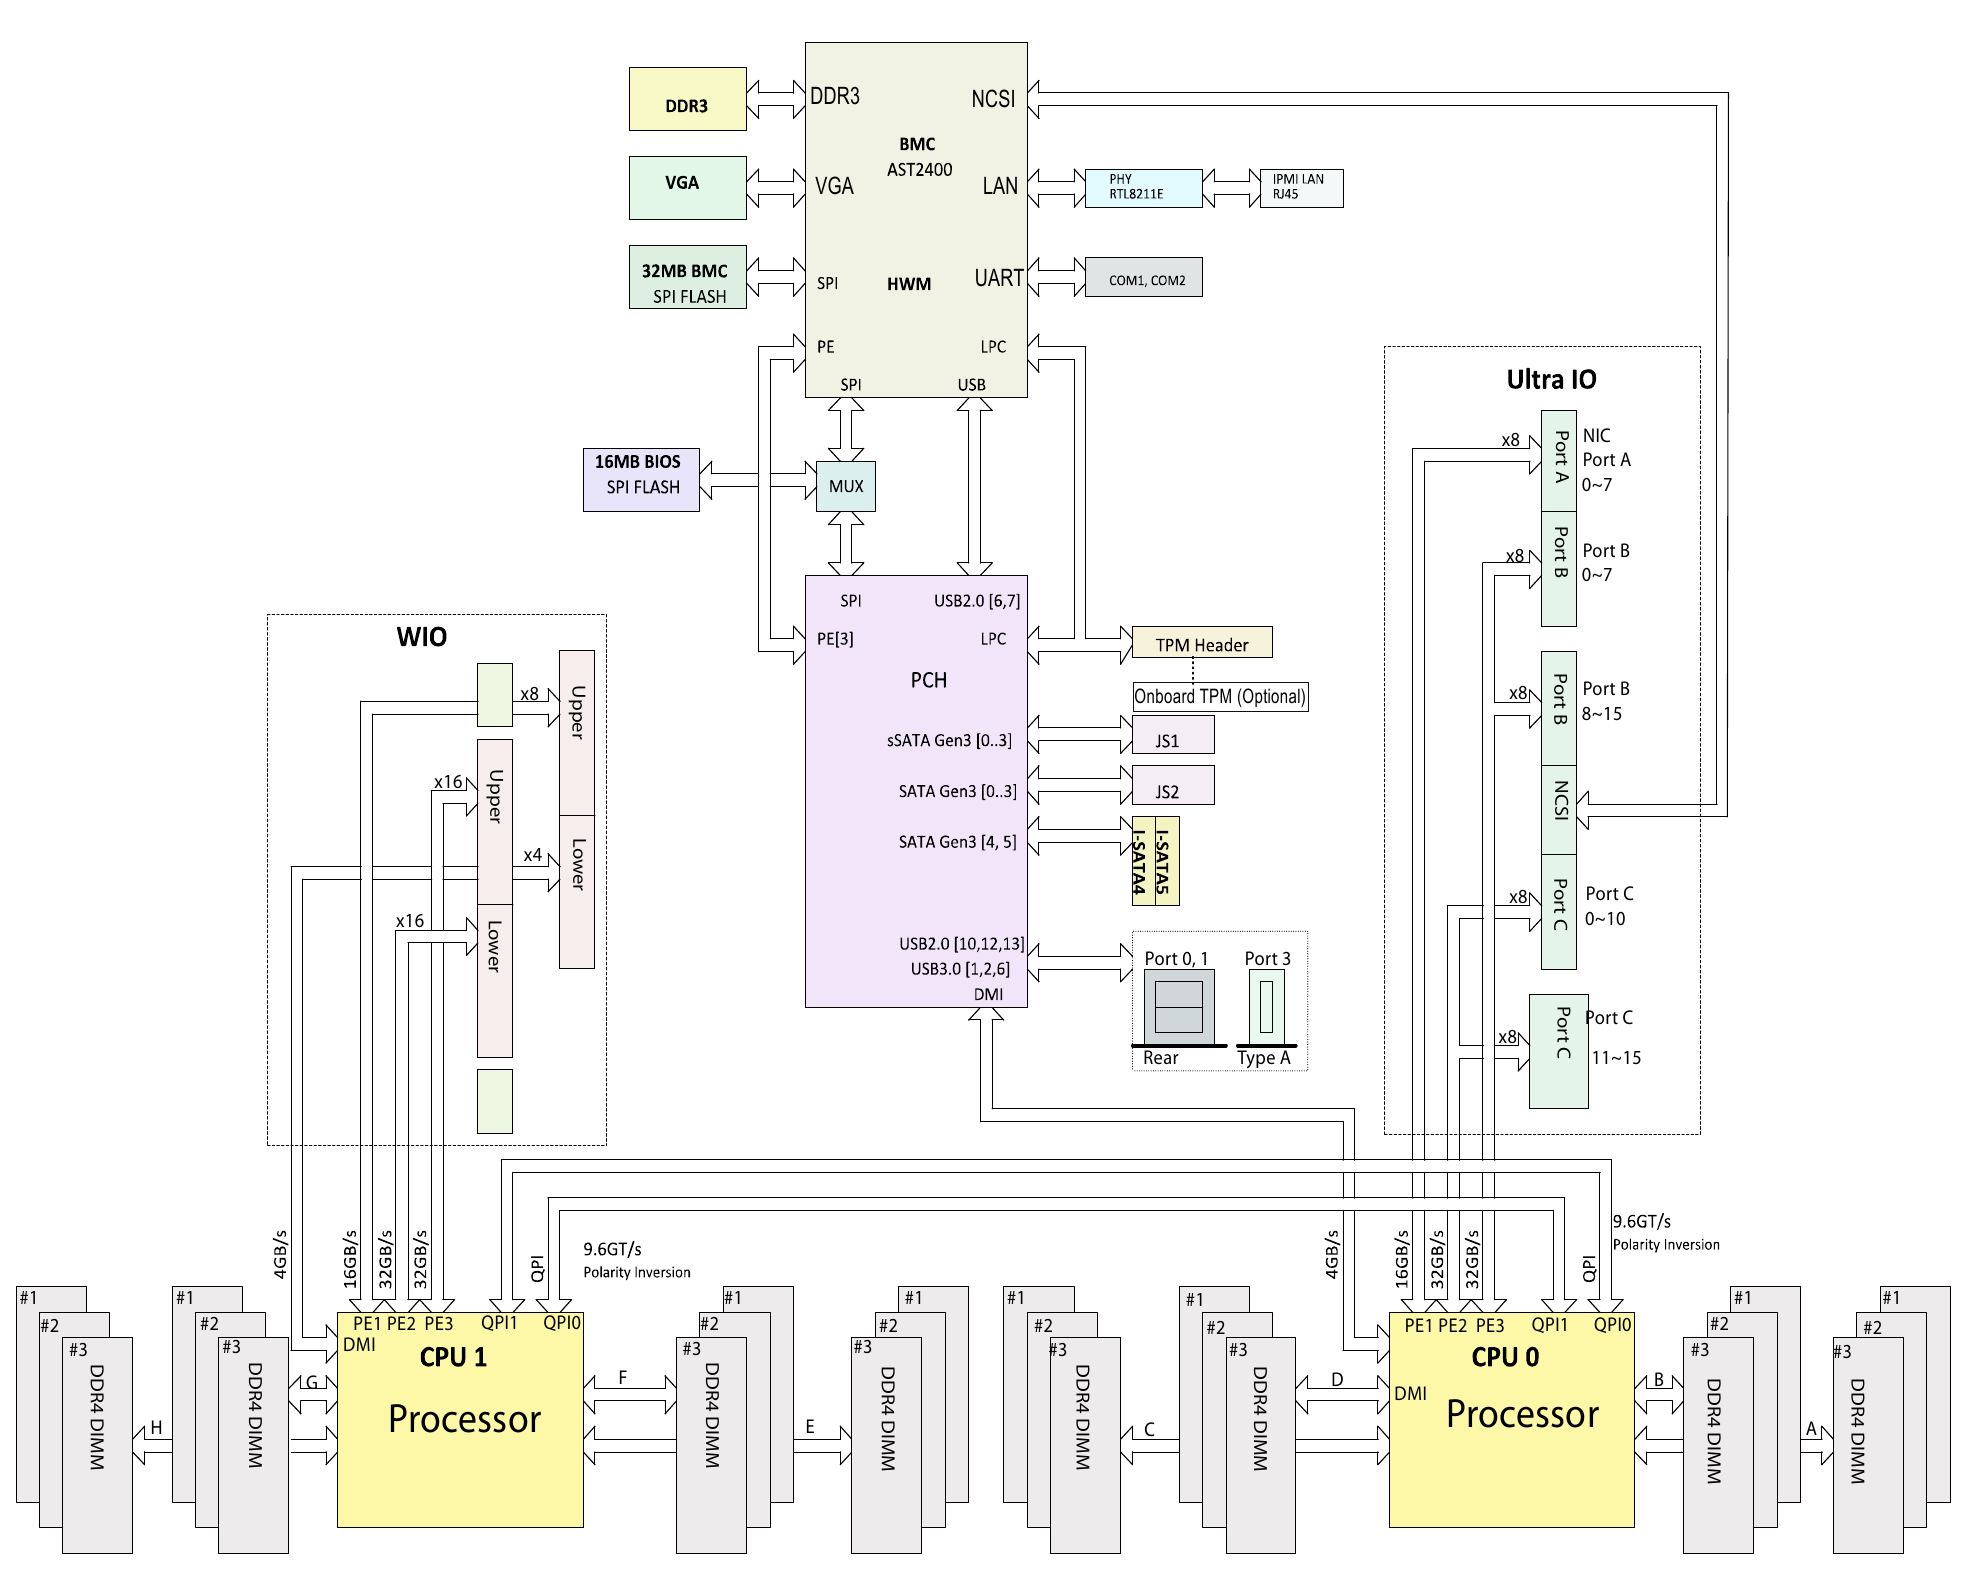
\includegraphics[width=15cm,keepaspectratio]{fig/supermicro-x10drui.png}
	\caption{Supermicro motherboard's block diagram}
	\label{fig:setup-supermicro-board}
\end{figure}

The server was put to the same rack as the Spirent hardware generator.
A pair of 2 metres long 40GBASE-SR4 multimode fiber cables with QSPF connectors
was used to connect Spirent with the Mellanox ConnectX-3 EN adapter.

IPv4 addresses from 192.0.2.0/24 (TEST-NET-1) block were assigned.
IPv6 addresses from 2001:db8::/32 range were assigned.
Addresses within these blocks should not appear on the public Internet
and therefore they do not conflict with the prefixes from the Internet BGP table~\cite{rfc3849}~\cite{rfc5737}.
Figure~\ref{fig:addressing-scheme} shows the addressing scheme used for the measurements.
\begin{figure}[H]
	\centering
	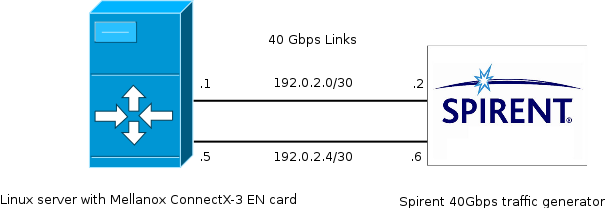
\includegraphics[width=13.5cm,keepaspectratio]{fig/net-setup.png}
	\caption{Addressing scheme}
	\label{fig:addressing-scheme}
\end{figure}



%Enable IPv4 packet forwarding:
%echo 1 > /proc/sys/net/ipv4/ip\_forward


%ip neigh add 1.0.0.2 lladdr f4:52:14:5e:6c:71 dev enp6s0d1
%ip neigh add 2.0.0.2 lladdr f4:52:14:5e:6c:70 dev enp6s0

%ip addr add 1.0.0.1/24 broadcast 1.0.0.255 dev enp6s0d1
%ip addr add 2.0.0.1/24 broadcast 2.0.0.255 dev enp6s0


%Load BGP routes:
%\begin{lstlisting}
%Basic info: size of leaf: 40 bytes, size of tnode: 40 bytes.
%Main:
        %Aver depth:     2.43
        %Max depth:      8
        %Leaves:         503308
        %Prefixes:       538739
        %Internal nodes: 114430
          %1: 58725  2: 26171  3: 14808  4: 7316  5: 4239  6: 2103  7: 1065  8: 2  17: 1
        %Pointers: 995798
%Null ptrs: 378061
%Total size: 61373  kB
%\end{lstlisting}
